\chapter{Le facteur $\alpha_L$ à l'initialisation}

Dans cette section, notre objectif est d'examiner comment le facteur de mise à l'échelle $\alpha_L$ affecte la stabilité des ResNets lors de leur initialisation, en supposant que les poids sont des variables aléatoires indépendantes et identiquement distribuées (i.i.d.). Nous analyserons la modélisation, l'initialisation des paramètres et les hypothèses nécessaires à cette démarche.
% Faire un horizon de la partie "related works" en creusant plus loin ? 

\section{Modèle et hypothèses}
\subsection*{Modèle}
Le modèle est basé sur un ensemble de données composé de $n$ paires $(x_i, y_i)_{1 \leq i \leq n}$ avec $x_i \in \mathbb{R}^{n_{\text{in}}}$ comme vecteur d'entrée et $y_i \in \mathbb{R}^{n_{\text{out}}}$ comme vecteur de sortie à prédire (soit en valeurs continues soit en format \textit{one-hot}). Soit $F_\pi(x) \in \mathbb{R}^{n_{\text{out}}}, x \in \mathbb{R}^{n_{\text{in}}}$ la sortie du ResNet définie par 
\begin{align}\label{ResNet_equation}
    h_0 &= Ax, \nonumber\\
    h_{k+1} &= h_k + \alpha_L V_{k+1}g(h_k, \theta_k), \quad 0 \leq k \leq L - 1, \\
    F_{\pi}(x) &= Bh_L, \nonumber
\end{align}
où $\pi = (A, B, (\theta_k)_{k \leq L}, (V_k)_{1 \leq k \leq L})$ sont les paramètres du modèle avec $A \in \mathbb{R}^{d \times n_{\text{in}}}, B \in \mathbb{R}^{n_{\text{out}} \times d}, \theta_k \in \mathbb{R}^p$ et $V_k \in \mathbb{R}^{d \times d}$ pour $k = 1, \ldots, L$. La fonction $g : \mathbb{R}^d \times \mathbb{R}^p \to \mathbb{R}^d$ représente le choix de l'architecture d'un bloc du ResNet. Nous nous intéressons principalement à la suite des états cachés $(h_k)_{0 \leq k \leq L}$ et non aux changements de dimension permis par les matrices $A$ et $B$.
% Un aspect important du modèle \cite{torchvision2016} est que la fonction de couche prend la forme d'une multiplication matrice-vecteur, ce qui sera crucial pour utiliser les résultats de concentration sur des variables aléatoires ??????? Important ????????? 
Finalement, on définit $l: \mathbb{R}^{n_{\text{out}}} \times \mathbb{R}^{n_{\text{out}}} \to \mathbb{R}_+$ comme la fonction de \textit{loss}, différentiable par rapport à son premier paramètre. Cette \textit{loss} peut être une perte quadratique ou une entropie croisée. L'objectif de l'apprentissage est de trouver le paramètre optimal $\pi$ qui minimise le risque empirique $\mathcal{L}(\pi) = \sum_{i=1}^{n} l(F_\pi(x_i), y_i)$ à travers une descente de gradient stochastique ou l'une de ses variantes.

Durant ce cours, nous nous concentrerons particulièrement sur trois architectures classiques de ResNet, présentées dans la \cref{tab:resnet_architectures} ci-dessous. Il pourrait également être intéressant d'envisager un quatrième modèle intégrant plusieurs couches linéaires ou convolutives.

\begin{table}[H]
    \centering
    \begin{tabular}{lll}
        \hline
        \textbf{Nom} & \textbf{Récurrence} & \textbf{Paramètres} \\ \hline
        res-1 & \( h_{k+1} = h_k + \alpha_L V_{k+1}\sigma(h_k) \) & \( \theta_{k+1} = \emptyset \) \\
        res-2 & \( h_{k+1} = h_k + \alpha_L V_{k+1}\sigma(W_{k+1}h_k) \) & \( \theta_{k+1} = W_{k+1} \) \\
        res-3 & \( h_{k+1} = h_k + \alpha_L V_{k+1}\text{ReLU}(W_{k+1}h_k) \) & \( \theta_{k+1} = W_{k+1} \) \\ \hline
    \end{tabular}
    \caption{Exemples d'architectures ResNet considérées dans l'article. Dans les deux premiers cas, la fonction d'activation \( \sigma \) est telle que, pour tout \( x \in \mathbb{R} \), \( a|x| \leq |\sigma(x)| \leq b|x| \), avec \( \frac{1}{\sqrt{2}} \leq a < b \leq 1 \). Dans les deux derniers cas, \( W_{k+1} \in \mathbb{R}^{d \times d} \).}
    \label{tab:resnet_architectures}
\end{table}

\subsection*{Initialisation des paramètres} 
Nous rappelons que $\theta_k \in \mathbb{R}^p$ et $V_k \in \mathbb{R}^{d \times d}$ sont les paramètres des couches cachées de notre modèle pour tout $k \in \llbracket 1, L \rrbracket$. Ces paramètres sont choisis à l'initialisation comme la réalisation de variables aléatoires i.i.d., généralement suivant une distribution uniforme ou gaussienne. Cette initialisation est indépendante de $L$ et donc du modèle représenté par $g$, permettant de considérer plusieurs architectures différentes dans notre étude. Nous examinerons également d'autres approches dépendantes du modèle pour étudier le choix de $\alpha_L$ (par exemple, Yang et Schoenholz, 2017 ou Wang et al., 2022 \cite{torchvision2016}).

\subsection*{Hypothèses}
Pour notre première hypothèse, nous avons besoin de la définition suivante :
\begin{definition}[Variable aléatoire $s^2$ sub-gaussienne]
    En théorie des probabilités, une distribution $s^2$ sub-gaussienne est une distribution de probabilité caractérisée par une décroissance rapide des queues de distribution. Bien qu'il existe de nombreuses définitions et propriétés, nous retiendrons dans ce cours la suivante : soit $X$ une variable aléatoire réelle,
    \[
        \forall \lambda \in \mathbb{R}, \mathbb{E}[\exp(\lambda X)] \leq \exp\left(\frac{\lambda^2 s^2}{2}\right).
    \]
    De manière informelle, les queues d'une distribution sub-gaussienne sont dominées par celles d'une distribution gaussienne, c'est-à-dire qu'elles décroissent au moins aussi rapidement.
\end{definition}

Avec cette définition en tête, passons aux hypothèses. Pour tout $ 1 \leq  k \leq L  $
\begin{assumption}\label{H1}
    Pour un certain $ s \geq 1 $, les entrées de  $ \sqrt{d}V_k $ sont des variables aléatoires symétriques i.i.d., $ s^2 $ sub-gaussiennes, indépendantes de $ d $ et $ L $ et de variance unitaire.
\end{assumption}
\begin{note}
    L'hypothèse \ref{H1} est en pratique satisfaite par toutes les initialisations, en particulier celle par défaut dans les paquets Keras \cite{chollet2015keras} et Torch Vision \cite{torchvision2016}.
    % Cette hypothèse permet de .... dans la preuve ... ?? Tant pis :’(
\end{note}

\begin{assumption}\label{H2}
    Pour un certain $ C > 0 $, indépendant de $ d $ et $ L $, et pour tout $ h \in \mathbb{R}^D  $ 
    \[
        \frac{\left\| h \right\| ^2}{2 } \leq  \mathbb{E }[ \left\|  g(h, \theta _ k ) \right\| ^2 ] \leq \left\| h \right\| ^2
    .\]
    and
    \[
        \mathbb{E } [\left\| g(h, \theta _k)  \right\| ^8 ]\leq C \left\| h  \right\| ^8
    .\]
\end{assumption}
\begin{note}
    La première partie de l'hypothèse \ref{H2} assure que $g(\cdot, \theta_{k+1})$ se comporte approximativement comme une isométrie en moyenne, c'est-à-dire qu'elle préserve les longueurs et les mesures d'angles entre son espace de départ et son espace d'arrivée.

    La deuxième partie de l'hypothèse \ref{H2} vise à limiter les variations excessives dans la norme de $g(h_k, \theta_{k+1})$.
\end{note}

\begin{proposition}[Admis]\label{prop1}
    Soit les modèles \textit{res-1}, \textit{res-2}, \textit{res-3} décrit dans la \Cref{tab:resnet_architectures}, on a \begin{itemize}
        \item [(i)] L'\Cref{H2} est valide pour l'architecture \textit{res-1}
        \item [(ii)] L'\Cref{H2} est valide pour les architectures \textit{res-2} et \textit{res-3} dès lors que les entrées de $ \sqrt{d}W_{k+1}, 0 \leq k \leq L-1 $ sont des variables aléatoire de variance unitaire, i.i.d., symétriques, sub-gaussienne et indépendante de $ d $ et $ L $
    \end{itemize}
\end{proposition}


\begin{lem}[Admis]\label{lem14}
    Considérons un ResNet [\ref{resnet_equation}] tel que les hypothèses \ref{H1} et \ref{H2} soient satisfaites.
    \[
        ((1 + \frac{\alpha _L ^2 }{2 }) ^L - 1) \leq \mathbb{E}( \frac{\left\| h_L - h_0 \right\| ^2 }{\left\| h_0 \right\| ^2}) \leq ((1 + \alpha _L ^2 ) ^L - 1 )
    .\]
\end{lem}
Ce lemme nous servira en particulier dans la preuve de la proposition \ref{prop2}.

\section{Limite probabilistique de la norme des états cachés}

Dans cette section, nous nous intéressons à la quantité $ {\left\| h_L - h_0 \right\|} / {\left\| h_0 \right\|}$. Cette mesure permet d'analyser la valeur des états cachés entre le début et la fin du réseau. Si $\left\| h_L - h_0 \right\| \ll \left\| h_0 \right\|$, cela suggère que le réseau agit presque comme une fonction identité. À l'inverse, un ratio $\left\| h_L - h_0 \right\| \gg \left\| h_0 \right\|$ indique une explosion des valeurs des états cachés. Une situation équilibrée serait représentée par $\left\| h_L - h_0 \right\| \approx \left\| h_0 \right\|$.

Nous appliquerons un raisonnement similaire aux gradients avec la quantité ${\left\| \frac{\partial \mathcal{L}}{\partial h_0} - \frac{\partial \mathcal{L}}{\partial h_L} \right\|} / {\left\| \frac{\partial \mathcal{L}}{\partial h_L} \right\|}$. En raison de la propagation rétroactive du gradient qui commence à partir de la fin du réseau, cette mesure est comparée à la dernière valeur du gradient $\frac{\partial \mathcal{L}}{\partial h_L}$.

Les propositions et corollaires suivants décriront comment le rapport ${\left\| h_L - h_0 \right\|} / {\left\| h_0 \right\|}$ se comporte en fonction de $L\alpha_L$, en établissant différentes bornes supérieures et inférieures.


\begin{proposition}\label{prop2}
    Considérons un ResNet [\ref{resnet_equation}] tel que les hypothèses \ref{H1} et \ref{H2} soient satisfaites.
    Si \( L\alpha_L^2 \leq 1 \), alors, pour tout \( \delta \in (0, 1) \), avec une probabilité d'au moins \( 1 - \delta \),
    \[
        \frac{\|h_L - h_0\|^2}{\|h_0\|^2} \leq \frac{2L\alpha_L^2}{\delta}
    .\]
\end{proposition}
La proposition \ref{prop2} par sa borne supérieur petite indique que le réseau se comporte comme une fonction identité dans le cas où $ L \alpha ^2 _L \ll 1 $.

\begin{proof}[\Cref{prop2}]
    En se basant sur le \cref{lem14}, on a 
    \[
        \mathbb{E}( \frac{\left\| h_L - h_0 \right\| ^2 }{\left\| h_0 \right\| ^2}) \leq ((1 + \alpha _L ^2 ) ^L - 1 )
    .\]
    En se basant sur le lemme \ref{lem14}, considérons le cas où $L \alpha_L^2 \leq 1$ (valeur faible) et $L$ tend vers de grandes valeurs. Dans ce contexte, $(1 + \alpha_L^2)^L$ est une bonne approximation de $\exp(L \alpha_L^2)$ par définition, tout en restant inférieur ou égal à celui-ci en raison de la croissance exponentielle de la fonction $\exp$. En effet, $(1 + \alpha_L^2)^L$ se rapproche de $1 + L \alpha_L^2$ selon la formule du binôme de Newton, et correspond aux premiers termes du développement en série de Taylor de l'exponentielle. Finalement, on a obtiens
    \[
        (1 + \alpha _L ^2)^L -1 \leq \exp (L \alpha _L ^2) - 1
    .\]
    En poursuivant avec le développement de Taylor, nous obtenons une majoration plus précise.
    \[
        (1 + \alpha _L ^2)^L -1 \leq \exp (L \alpha _L ^2) - 1) \leq L \alpha _L ^2 \leq 2 L \alpha _L ^2
    .\]
    Ainsi on obtient 
    \[
        \mathbb{E}( \frac{\left\| h_L - h_0 \right\| ^2 }{\left\| h_0 \right\| ^2}) \leq 2 L \alpha _L ^2
    .\]
    En appliquant l'inégalité de Markov, nous parvenons au résultat souhaité.
\end{proof}



\begin{proposition}[Admise]\label{prop3}
    Considérons un ResNet [\ref{resnet_equation}] tel que les hypothèses \ref{H1} et \ref{H2} soient satisfaites.
    \begin{itemize}
        \item[(i)] Supposons que $ d \geq 64 $ et $ \alpha _L ^2 \leq  \frac{2 }{(\sqrt{C } s^4 + 4 \sqrt{C } + 16 s ^4)d} $. Alors, pour tout $ \delta \in (0, 1) $, avec une probabilité d'au moins $ 1 - \delta $,
        \[
            \frac{\|h_L - h_0\|^2}{\|h_0\|^2} > \exp\left(\frac{3L\alpha_L^2}{8} - \sqrt{\frac{11L\alpha_L^2}{d\delta}}\right) - 1,
        \]
        à condition que
        \[
            2L \exp\left(-\frac{d}{64\alpha_L^2s^2}\right) \leq \frac{\delta}{11}.
        \]
        \item[(ii)] Supposons que $ \alpha_L^2 \leq \frac{1}{\sqrt{C}(d + 128s^4)} $. Alors, pour tout $ \delta \in (0, 1)$, avec une probabilité d'au moins $1 - \delta $,
        \[
            \frac{\|h_L - h_0\|^2}{\|h_0\|^2} < \exp\left(L\alpha_L^2 + \sqrt{\frac{5L\alpha_L^2}{d\delta}}\right) + 1.
        \]
    \end{itemize}
\end{proposition}
La proposition \ref{prop3} aborde les deux cas restants : $L \alpha_L^2 \gg 1$ et $L \alpha_L^2 \approx 1$. Dans la partie \textit{(i)}, la borne inférieure indique une explosion très probable du gradient lorsque $L \alpha_L^2 \gg 1$. La partie \textit{(ii)} traite du cas où $L \alpha_L^2 \approx 1$, avec une borne supérieure qui, en combinaison avec celle de \textit{(i)}, suggère que $h_L$ fluctue autour de $h_0$, étant ainsi borné des deux côtés.

Cette proposition \ref{prop3} peut présenter des hypothèses qui semblent atypiques, mais elles sont en réalité souvent vérifiées dans la majorité des ResNets profonds. En effet, il est courant de trouver des ResNets avec une profondeur $L \geq 100$, pour lesquels on définit généralement $\alpha_L = 1 / L^\beta$ avec $\beta > 0$. De plus, la dimension des états cachés atteint fréquemment des valeurs telles que $d \geq 100$.

Les conséquences des propositions \ref{prop2} et \ref{prop3} vont devenir plus clair en fixant $ \alpha _L = 1/L ^\beta $ comme montré dans le corollaire suivant.
\begin{cor}\label{cor4}
    Considérons un ResNet [\ref{resnet_equation}] tel que les hypothèses \ref{H1} et \ref{H2} soient satisfaites, et soit $ \alpha_L = 1/L^\beta $, avec $ \beta > 0 $.
    \begin{itemize}
        \item[(i)] Si $ \beta > \frac{1}{2} $, alors
        \[
            \frac{\|h_L - h_0\|}{\|h_0\|} \xrightarrow{\mathbb{P}} 0 \text{ lorsque } L \to \infty.
        \]
        \item[(ii)] Si $ \beta < \frac{1}{2}$ et $d \geq 9 $, alors
        \[
            \frac{\|h_L - h_0\|}{\|h_0\|} \xrightarrow{\mathbb{P}} \infty \text{ lorsque } L \to \infty.
        \]
        \item[(iii)] Si $ \beta = \frac{1}{2} $, $ d \geq 64$, $L \geq \left(\frac{1}{2}\sqrt{C}s^4 + 2\sqrt{C} + 8s^4)d + 96\sqrt{C}s^4\right) $, alors, pour tout $ \delta \in (0, 1) $, avec une probabilité d'au moins $ 1 - \delta $,
        \[
            \exp\left(\frac{3}{8} - \sqrt{\frac{22}{d\delta}}\right) - 1 < \frac{\|h_L - h_0\|^2}{\|h_0\|^2} < \exp\left(1 + \sqrt{\frac{10}{d\delta}}\right) + 1,
        \]
        à condition que
        \[
            2L \exp\left(-\frac{Ld}{64s^2}\right) \leq \frac{\delta}{11}.
        \]
    \end{itemize}
\end{cor}
Le corollaire 4 clarifie le comportement de notre dernier état caché $ \left\| h_L \right\|  $ en fonction de $ \beta  $. 
\begin{itemize}
    \item Lorsque $ \beta > 1/2 $, la distance entre $ h_L $ et $ h_0 $ converge vers zéro lorsque $ L $ tend vers l'infinie. Indiquant un réseau aggisant essentiellement comme une fonction identité.
    \item Lorsque $ \beta < 1/2 $, la norme de $ h_L $ explose.
    \item Lorsque $ \beta = 1/2 $, On voit que $ h_L $ fluctue autour de $ h_0 $, indépendament de la longueur du réseau $ L $.
\end{itemize}
On conclu donc que seul fixer $ \beta = 1/2 $ permet d'obtenir une distribution correcte.

Le corollaire 4 précise le comportement de notre dernier état caché $\left\| h_L \right\|$ en fonction de $\beta$.
\begin{itemize}
    \item Lorsque $\beta > 1/2$, la distance entre $h_L$ et $h_0$ tend vers zéro lorsque $L$ augmente indéfiniment. Cela indique que le réseau fonctionne essentiellement comme une fonction identité.
    \item Lorsque $\beta < 1/2$, la norme de $h_L$ tend à l'explosion avec la valeur de $ L $ .
    \item Lorsque $\beta = 1/2$, $h_L$ fluctue autour de $h_0$, indépendamment de la longueur du réseau $L$.
\end{itemize}
En conséquence, fixer $\beta = 1/2$ est la seule manière d'assurer une distribution adéquate des valeurs de $h_L$.


\begin{proof}[\Cref{cor4}]
    L'affirmation ($ i $) est une conséquence de la Proposition \ref{prop2}.
    % Tentative de preuve......
    %%%%%%%%%%%%%%%%%%%%%%%%%%%%%%%%%%%%%%%%%%%%
    % Nous avons $ L \alpha _L ^2 = \frac{L}{L^{2\beta} } = L^{1 - 2 \beta } $, comme $ \beta > 1/2 \Leftrightarrow 1 - 2 \beta < 0 $ nous avons $ L^{1 - 2 \beta } = \frac{1}{L^{2 \beta  -1}} \underset{L\to +\infty}{\longrightarrow} 0 $. Ainsi
    % \begin{align*}
    %     & \frac{\|h_L - h_0\|^2}{\|h_0\|^2} \leq \frac{2L\alpha_L^2}{\delta}.
    %     \overunderset{\mathbb{P}}{L\to +\infty}{\longrightarrow} 0 
    % \end{align*}
    %%%%%%%%%%%%%%%%%%%%%%%%%%%%%%%%%%%%%%%%%%%%
    L'affirmation ($ ii $) est une conséquence de la \Cref{prop3}. En effet, cette dernière est valide les conditions $ d \geq 64 $ et $ \alpha _L \leq \frac{2}{(\sqrt{C} s^4 + 4 \sqrt{C} + 16s^4)d} $. La majoration d'$ \alpha _L $ est automatiquement satisfaite pour $ L $ assez grand. Quant à la contrainte sur $ d $, elle peut être, dans notre cas, relaché à $ d \geq 9 $ en observant la preuve de la \Cref{prop3} non décrite ici.

    Pour prouver l'affirmation $ (iii) $, nous utilisons l'union des deux affirmations ce la \Cref{prop3}.
    % TODO better sentences
\end{proof}

\begin{figure}[H]
    \centering
    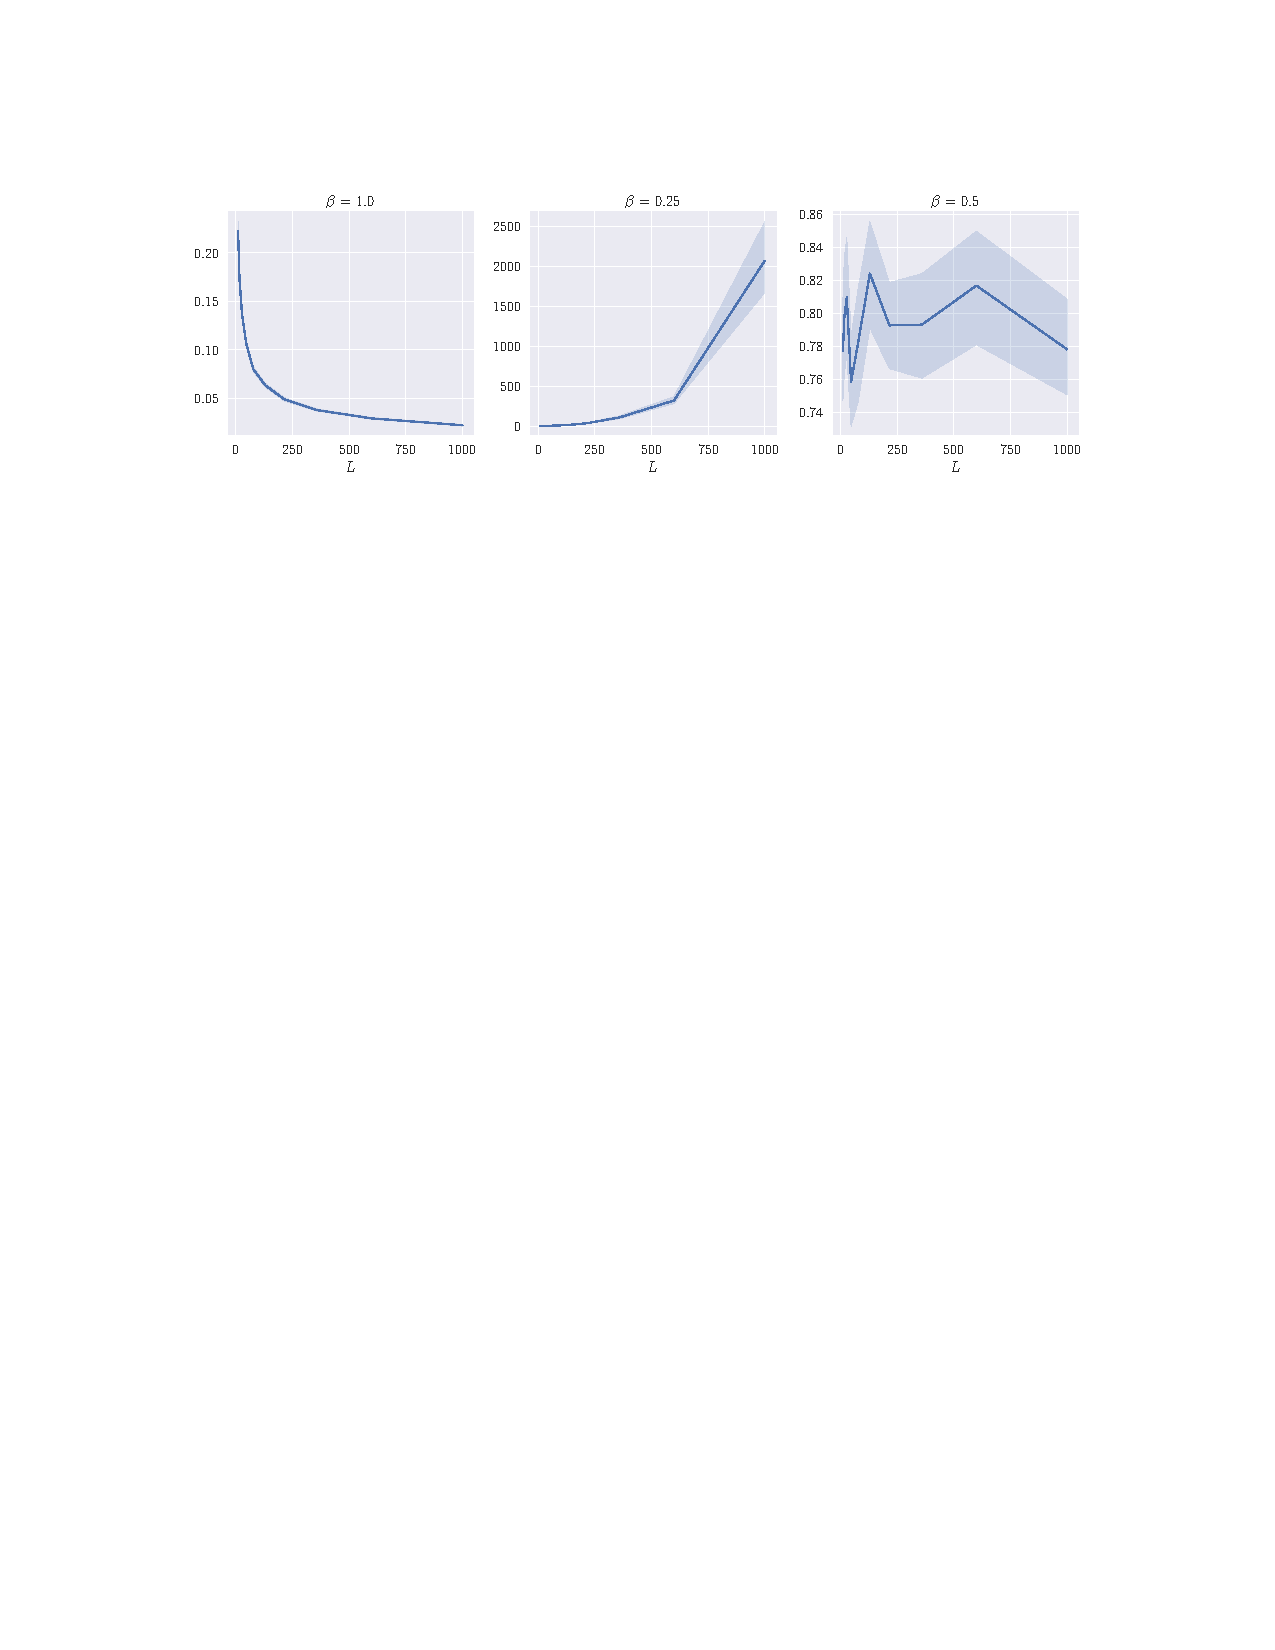
\includegraphics[width=.95\textwidth]{figs/figure_cor4.pdf}
    \caption{Illustration du corollaire \ref{cor4}. Évolution de $ \left\| h_L - h_0 \right\| / \left\| h_0 \right\| $ en fonction de $ L $ pour différente valeur de $ \beta  $.}
    \label{fig:cor4}
\end{figure}

